\RequirePackage{plautopatch}
\documentclass[uplatex,a4paper,11pt,dvipdfmx]{jsreport}

\usepackage{bm}
\usepackage{physics}
\usepackage[dvipdfmx]{graphicx}
\usepackage{here}
\usepackage[utf8]{inputenc}
\usepackage{tcolorbox}
\tcbuselibrary{breakable,theorems}
\usepackage{tikz}
\usetikzlibrary{intersections, calc, arrows.meta}
\usepackage{amsmath}
\usepackage{titleps}
\usepackage{enumerate}
\usepackage{amsfonts}
\usepackage{amssymb}
\usepackage{wrapfig}
\usepackage{ascmac}
\usepackage{siunitx}
\usepackage{cancel}
% \usepackage{udline}
\usepackage[hang,small,bf]{caption}
\usepackage[subrefformat=parens]{subcaption}
\usepackage{import}
\usepackage{color}
\usepackage{okumacro}
\usepackage{framed}
\usepackage{hyperref}
\usepackage{pxjahyper}
\usepackage{booktabs}
\usepackage{algpseudocode}
\usepackage{algorithm}
\usepackage{natbib}
\usepackage{mathtools}
\usepackage{longtable}
\usepackage{subfiles}
\bibpunct{(}{)}{;}{a}{}{,}

\hypersetup{% hyperrefオプションリスト
    setpagesize=false,
    bookmarksnumbered=true,%
    bookmarksopen=true,%
    colorlinks=true,
    linkcolor=blue,
    citecolor=blue,
    urlcolor=blue
}

\setlength{\textwidth}{\fullwidth}  %本文の幅(textwidth)を全体の幅(=ヘッダ部の幅)にそろえる
\setlength{\evensidemargin}{\oddsidemargin} %偶数ページの余白と奇数ページの余白をそろえる

\title{\textbf{宇宙論的シミュレーションデータベースIllustris-TNGを用いた銀河周辺物質の速度と元素分布構造の解明}}
\author{埼玉大学理学部物理学科 \\ 宇宙物理実験研究室 \\ \\ 20RP021 西濱大将}
\date{2024/02/xx}


\begin{document}
    \maketitle
    \begin{abstract}
    あ
\end{abstract}
    \setcounter{tocdepth}{2}
    \tableofcontents
    \subfile{introduction}
    \subfile{method}
    \subfile{result}
%    \documentclass[main.tex]{subfiles}
\begin{document}
	\chapter{議論}
	\section{subhalo342447における$\mathrm{[X/Fe]} > 0$について}

図\ref{fig:fe10}に示すように,X $=$ Ne, O, Mg, Siとして$\mathrm{[X/Fe]} > 0$がいえる.このようなXをアルファ($\alpha$)元素という.中性子数と陽子数が偶数で等しく,$\alpha$粒子(\ce{^{4}He})の集まりと見なせることから,この名前で呼ばれている.Feよりもアルファ($\alpha$)元素が多いということは,アルファ($\alpha$)元素の生成元される重力崩壊型超新星爆発(II型超新星爆発)に由来するものと考えられる.

II型超新星の中心部では核融合反応が進行し,アルファ($\alpha$)元素を生成する.核融合のエネルギーと重力が平衡状態であったのが,鉄まで生成されると平衡状態が崩れ,収縮を始める.中心核は中性子の縮退圧と重力が枯渇すると急停止し,上層は中心核によって反跳し衝撃波が発生する.ゆえに大量のアルファ($\alpha$)元素を宇宙空間にばらまくことになる.

\section{アウトフローと太陽組成比との関係}

アウトフローが観測されたsubhalo342447は図\ref{fig:abundanceprofile342447}に示したように,R/R$_{200} < 0.1$において太陽組成の2倍近くFe, O, Mg, Siなどの元素が観測された.一方でアウトフローが観測されなかったsubhalo388544やsubhalo421555はR/R$_{200} < 0.1$において太陽組成程度であることが観測された(図\ref{fig:2radicalprofile}).

このようなことからアウトフローと太陽組成には何らかの因果関係がある可能性がある.

\section{subhalo342447の「へこみ」と温度分布の高温部}

図\ref{fig:fe10}において$0.1<\text{R/R}_{200} < 0.5$で他の部分と組成が異なる「へこみ」が観測されたことに加え,図\ref{fig:atemp}の右側で,R/R$_{200} < 0.1$においては\SI{e6}{K}以上の高温ガスが確認できたことから,subhalo342447が現在の状態になるまでに,他のsubhaloと衝突をし,そのsubhaloの組成の一部を取り込んだ可能性が考えられる.

\begin{figure}[htbp]
	\centering
	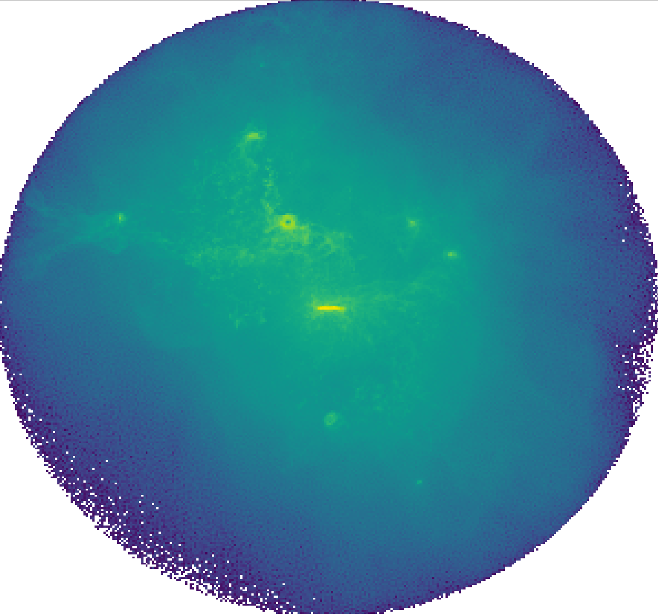
\includegraphics[width=0.6\linewidth]{pic/virial3}
	\captionsetup{width=0.9\linewidth}
	\caption{subhalo342447をedge-onにした状態で中心にとり,ビリアル半径の3倍を表示.濃淡は対数で質量を表す.}
	\label{fig:virial3}
\end{figure}

また図\ref{fig:virial3}に示すようにsubhalo342447の周囲に別のsubhaloが観測され,ガスの散乱具合も衝突後のような状態となっている.このようなことから衝突した可能性は非常に高いと考えられる.
\end{document}
%    \chapter{まとめ}
%    \chapter*{謝辞}
\addcontentsline{toc}{chapter}{謝辞}


    \nocite{*}
    \bibliographystyle{aasjournal}
    \bibliography{res2023}
    \addcontentsline{toc}{chapter}{\bibname}
    
    \subfile{appendix}
\end{document}